% 本LaTeX模板的使用示例
\chapter{示例}
%==============================
\section{参考文献引用}
测试一下上标引用\upcite{Ruel_2012},引用\cite{knuth84,knuth86a,lamport94},还有其它引用\upcite{Ruel_2012,knuth86a,lamport94}.
%--------------------------------
\subsection{数字标注}
\noindent
\begin{tabular}{l@{\quad$\Rightarrow$\quad}l}
  \verb|\cite{knuth86a}| & \cite{knuth86a}\\
  \verb|\citet{knuth86a}| & \citet{knuth86a}\\
  \verb|\citet[chap.~2]{knuth86a}| & \citet[chap.~2]{knuth86a}\\[0.5ex]
  \verb|\citep{knuth86a}| & \citep{knuth86a}\\
  \verb|\citep[chap.~2]{knuth86a}| & \citep[chap.~2]{knuth86a}\\
  \verb|\citep[see][]{knuth86a}| & \citep[see][]{knuth86a}\\
  \verb|\citep[see][chap.~2]{knuth86a}| & \citep[see][chap.~2]{knuth86a}\\[0.5ex]
  \verb|\citet*{knuth86a}| & \citet*{knuth86a}\\
  \verb|\citep*{knuth86a}| & \citep*{knuth86a}\\
\end{tabular}
\par\noindent
\begin{tabular}{l@{\quad$\Rightarrow$\quad}l}
  \verb|\citet{knuth86a,tlc2}| & \citet{knuth86a,tlc2}\\
  \verb|\citep{knuth86a,tlc2}| & \citep{knuth86a,tlc2}\\
  \verb|\cite{knuth86a,knuth84}| & \cite{knuth86a,knuth84}\\
  \verb|\upcite{knuth86a,knuth84}| & \upcite{knuth86a,knuth84}\\
  \verb|\citet{knuth86a,knuth84}| & \citet{knuth86a,knuth84}\\
  \verb|\citep{knuth86a,knuth84}| & \citep{knuth86a,knuth84}\\
  \verb|\cite{knuth86a,knuth84,tlc2}| & \cite{knuth86a,knuth84,tlc2}\\
\end{tabular}

%--------------------------------
\subsection{数字标注-上标形式}
\noindent
\begin{tabular}{l@{\quad$\Rightarrow$\quad}l}
  \verb|\upcite{knuth86a}| & \upcite{knuth86a}\\
  \verb|\upcite{knuth86a,knuth84,tlc2}| & \upcite{knuth86a,knuth84,tlc2}\\
\end{tabular}
\par\noindent
实现源码:\verb|\newcommand{\upcite}[1]{\textsuperscript{\cite{#1}}}|。


%--------------------------------
\subsection{著者-出版年制标}
\citestyle{authoryear}
\noindent
\begin{tabular}{l@{\quad$\Rightarrow$\quad}l}
  \verb|\cite{knuth86a}| & \cite{knuth86a}\\
  \verb|\citet{knuth86a}| & \citet{knuth86a}\\
  \verb|\citet[chap.~2]{knuth86a}| & \citet[chap.~2]{knuth86a}\\[0.5ex]
  \verb|\citep{knuth86a}| & \citep{knuth86a}\\
  \verb|\citep[chap.~2]{knuth86a}| & \citep[chap.~2]{knuth86a}\\
  \verb|\citep[see][]{knuth86a}| & \citep[see][]{knuth86a}\\
  \verb|\citep[see][chap.~2]{knuth86a}| & \citep[see][chap.~2]{knuth86a}\\[0.5ex]
  \verb|\citet*{knuth86a}| & \citet*{knuth86a}\\
  \verb|\citep*{knuth86a}| & \citep*{knuth86a}\\
\end{tabular}
\par\noindent
\begin{tabular}{l@{\quad$\Rightarrow$\quad}l}
  \verb|\citet{knuth86a,tlc2}| & \citet{knuth86a,tlc2}\\
  \verb|\citep{knuth86a,tlc2}| & \citep{knuth86a,tlc2}\\
  \verb|\cite{knuth86a,knuth84}| & \cite{knuth86a,knuth84}\\
  \verb|\citet{knuth86a,knuth84}| & \citet{knuth86a,knuth84}\\
  \verb|\citep{knuth86a,knuth84}| & \citep{knuth86a,knuth84}\\
\end{tabular}
\citestyle{numbers}

%--------------------------------
\subsection{其他形式的标注}
\noindent
\begin{tabular}{l@{\quad$\Rightarrow$\quad}l}
  \verb|\citealt{tlc2}| & \citealt{tlc2}\\
  \verb|\citealt*{tlc2}| & \citealt*{tlc2}\\
  \verb|\citealp{tlc2}| & \citealp{tlc2}\\
  \verb|\citealp*{tlc2}| & \citealp*{tlc2}\\
  \verb|\citealp{tlc2,knuth86a}| & \citealp{tlc2,knuth86a}\\
  \verb|\citealp[pg.~32]{tlc2}| & \citealp[pg.~32]{tlc2}\\
  \verb|\citenum{tlc2}| & \citenum{tlc2}\\
  \verb|\citetext{priv.\ comm.}| & \citetext{priv.\ comm.}\\
\end{tabular}

\noindent
\begin{tabular}{l@{\quad$\Rightarrow$\quad}l}
  \verb|\citeauthor{tlc2}| & \citeauthor{tlc2}\\
  \verb|\citeauthor*{tlc2}| & \citeauthor*{tlc2}\\
  \verb|\citeyear{tlc2}| & \citeyear{tlc2}\\
  \verb|\citeyearpar{tlc2}| & \citeyearpar{tlc2}\\
\end{tabular}

\section{浮动体\footnote{样例参考《浙江大学研究生硕士(博士)学位论文\LaTeX{}模板》}}
在实际撰写文稿的过程中,我们可能会碰到一些占据篇幅较大,但同时又不方便分页的内容。(比如图片和表格,通常属于这样的类型)此时,我们通常会希望将它们放在别的地方,避免页面空间不够而强行置入这些内容导致 overfull vbox 或者大片的空白。此外,因为被放在别的地方,所以,我们通常需要对这些内容做一个简单的描述,确保读者在看到这些大块的内容时,不至于无从下手去理解。同时,因为此类内容被放在别的地方,所以在文中引述它们时,我们无法用「下图」、「上表」之类的相对位置来引述他们。于是,我们需要对它们进行编号,方便在文中引用。

在 \LaTeX{} 中,默认有 figure 和 table 两种浮动体。(当然,你还可以自定义其他类型的浮动体)在这些环境中,可以用 $\backslash$caption\{\} 命令生成上述简短的描述。至于编号,也是用 $\backslash$caption\{\} 生成的。这类编号遵循了 TeX 对于编号处理的传统:它们会自动编号,不需要用户操心具体的编号数值。 至于「别的地方」是哪里,\LaTeX{} 为浮动体启用了所谓「位置描述符」的标记。基本来说,包含以下几种:

h - 表示 here。此类浮动体称为文中的浮动体(in-text floats)。

t - 表示 top。此类浮动体会尝试放在一页的顶部。

b - 表示 bottom。此类浮动体会尝试放在一页的底部。

p - 表示 float page,浮动页。此类浮动体会尝试单独成页。

\LaTeX{} 会将浮动体与文本流分离,而后按照位置描述符,根据相应的算法插入 \LaTeX{} 认为合适的位置。

\subsection{插图测试}
如图\ref{fig:first_image_tset}是对此模版的第一张插图测试。

\begin{figure}[htbp]
	\centering
	
\includegraphics[width = 0.5\linewidth]{Chapter1.png}
	\caption{第一张插图测试}\label{fig:first_image_tset}
\end{figure}

以下是一段对这些插图来历的介绍,引用自知乎专栏All about TeXnique中夏晓昊的文章\href{http://zhuanlan.zhihu.com/LaTeX/19669122}{《The TeXbook导读:从那头(多图杀猫的)狮子说起》}。

在The TeXbook中,有着一系列的以狮子为主题的插图。这些插图的作者是Duane Bibby。也是从The TeXbook开始,不少TeX书也采取了以狮子为主的插图,作者也是Duane Bibby。另外,每年的TUG(TeX Users Group)年会都会有一张以狮子为主题的logo,这只狮子已经是社区的吉祥物了。

为什么选择狮子呢?Yannis Haralambous写道(原文法语,此为转译后的英文):Not for nothing is TeX represented by a lion. Donald Knuth has told us that lions are to him the guardians of libraries in the United States because there is a statue of a lion in front of the entrance of each large library there. Guardian of libraries, guardian of the Book—is that not indeed what TeX ultimately aspires to be? 或许吧。 (顺便说一句,TeX和MetaFont都用了狮子,TeX是公狮子,MetaFont是母狮子,多么和谐的一对啊。如果你还是忽略MetaFont的存在,那你还没有认识到它的重要性。)

作为插图,首要的一点就是贴切,然后是有趣。在TeX社区里面,have fun是一个很重要的词组,也有人说Happy TeXing。我知道有不少人不喜欢TeX,但是能有什么理由呢?如果你用不到它,那么浅尝辄止即可。如果你会用到很频繁,最好慢慢修炼做到精通。如果你只是偶尔用到,那么可以搬个模版什么的,甚至也可以找人帮你(不要指望别人会用足够的空闲时间来帮你,他没有这个义务,请支付报酬,最少也得请吃个饭吧)。下面的插图,是TeX TeXbook中的,我也希望这个假期,能有人有空来看看这本书。即使不能把所有的东西都看懂,那么也会对TeX的设计有了一定的了解,拿到扳手就好。

\subsection{表格测试}
在这里推荐制表采用功能强大的tabu宏包以取代其它制表宏包。具体tabu宏包的使用说明参见tabu宏包的说明文档。

以下节分别用来测试各种表格环境如,tabular,tabu,longtabu等,还有对caption格式的修改和测试。以下表格样式全部采用三线表。

\subsection{array宏包tabular表格环境测试}
如表\ref{tab:first_table_test}是对array宏包的tabular表格环境测试。
\begin{table}[htbp]
	\centering
	\caption{这是一个用tabular环境的测试用的表格}\label{tab:first_table_test}
	\begin{tabular}{lrr}
		\toprule
		\textbf{行星}     & \textbf{赤道半径}km & \textbf{公转周期}d \\
		\midrule
		水星     & 2.439  & 87.9 \\
		金星     & 6.1    & 224.682 \\
		地球     & 6378.14 & 365.24 \\
		\bottomrule
	\end{tabular}%
\end{table}

\subsection{tabu宏包表格环境测试}
如表\ref{tab:tabu_test_1}是对tabu宏包的tabu表格环境测试。在这里表格命令与表\ref{tab:first_table_test}的命令相同,只是tabular环境改成了tabu环境。
\begin{table}[htbp]
	\centering
	\caption{这是一个用tabu环境的测试用的表格}\label{tab:tabu_test_1}
	\begin{tabu}{lrr}
		\toprule
		\textbf{行星}     & \textbf{赤道半径}km & \textbf{公转周期}d \\
		\midrule
		水星     & 2.439  & 87.9 \\
		金星     & 6.1    & 224.682 \\
		地球     & 6378.14 & 365.24 \\
		\bottomrule
	\end{tabu}%
\end{table}

表\ref{tab:tabu_test_2}对tabu to表格的x列模式进行测试。在表格导言区中设置为X[1]X[2]X[2],表示这三列表格的列宽比值为1:2:2,总的表格宽度由tabu to环境设置,这里设置为0.6\textbackslash linewidth。相比于tabular环境,tabu环境的列宽设置方便许多。
\begin{table}[htbp]
	\centering
	\caption{tabu环境测试表格---X列模式}\label{tab:tabu_test_2}
	\begin{tabu} to 0.6\linewidth{X[1]X[2]X[2]}
		\toprule
		\textbf{行星}     & \textbf{赤道半径}km & \textbf{公转周期}d \\
		\midrule
		水星     & 2.439  & 87.9 \\
		金星     & 6.1    & 224.682 \\
		地球     & 6378.14 & 365.24 \\
		\bottomrule
	\end{tabu}%
\end{table}

如表\ref{tab:tabu_test_3}是longtabu环境测试表格。longtabu环境不能用在table浮动体环境中。根据GB/T 7713.1-2006规定:如果某个表需要转页接排,在随后的各页上应重复表的编号。编号后跟标题(可省略)和“(续)”,置于表上方。续表应重复表头。

特别需要注意的是,longtabu是基于longtable宏包开发的,所以在nmu.cls文件中已经插入了longtable宏包。longtable环境的所有功能都可以在longtabu中使用,如\textbackslash endhead,\textbackslash endfirsthead,\textbackslash endfoot,\textbackslash endlastfoot,和\textbackslash caption等。具体用法请参见longtable和tabu宏包的相应文档。
\begin{longtabu}{cccccc}
	\caption{2018年6月全球编程语言TIOBE排行榜}\label{tab:tabu_test_3}\\
	\toprule
	Jun 2018   & Jun 2017 & Change & Programming Language & Ratings &Change\\
	\midrule%
	\endfirsthead
	\caption{2018年6月全球编程语言TIOBE排行榜(续)}\\
	\toprule
	Jun 2018   & Jun 2017 & Change & Programming Language & Ratings &Change \\
	\midrule%
	\endhead
	\bottomrule%
	\endfoot
	1 & 1 &              & Java & 15.368$\%$ & +0.88$\%$  \\
	2 & 2 &              & C & 14.936$\%$ & +8.09$\%$  \\
	3 & 3 &              & C++ & 8.337$\%$ & +2.61$\%$  \\
	4 & 4 &              & Python & 5.761$\%$ & +1.43$\%$  \\
	5 & 5 &              & C$\#$ & 4.314$\%$ & +0.78$\%$  \\
	6 & 6 &              & Visual Basic .NET & 3.762$\%$ & +0.65$\%$  \\
	7 & 8 &   $\uparrow$ & PHP & 2.881$\%$ & +0.11$\%$  \\
	8 & 7 & $\downarrow$ & JavaScript & 2.495$\%$ & -0.53$\%$  \\
	9 & - &   $\uparrow$ & SQL & 2.339$\%$ & +2,34$\%$  \\
	10 & 14 & $\uparrow$ & R & 1.452$\%$ & -0.70$\%$  \\
	11 & 11 &  & Ruby & 1.253$\%$ & -0.97$\%$  \\
	12 & 18 & $\uparrow$ & Objective-C & 1.181$\%$ & -0.78$\%$  \\
	13 & 16 & $\uparrow$ & Visual Basic & 1.154$\%$ & -0.86$\%$  \\
	14 & 9 & $\downarrow$ & Perl & 1.147$\%$ & -1.16$\%$  \\
	15 & 12 & $\downarrow$ & Swift & 1.145$\%$ & -1.06$\%$  \\
	16 & 10 & $\downarrow$ & Assembly language & 0.915$\%$ & -1.34$\%$  \\
	17 & 17 &  & MATLAB & 0.894$\%$ & -1.10$\%$  \\
	18 & 15 & $\downarrow$ & Go & 0.879$\%$ & -1.17$\%$  \\
	19 & 13 & $\downarrow$ & Delphi/Object Pascal & 0.875$\%$ & -1.28$\%$  \\
	20 & 20 &  & PL/SQL & 0.848$\%$ & -0.72$\%$  \\
\end{longtabu}%

\subsection{子图}
这里子图的排版推荐使用subcaption宏包,不再推荐使用subfig宏包,更不推荐使用subfigure宏包。值得注意的是,在nmu.cls文件中已经写入了subcaption宏包,而且subcaption宏包与subfigure和subfig宏包是相互冲突的。因此,如果你还想使用subfig宏包而不想使用subcaption宏包,请自己到nmu.cls文件的相关位置更改,具体的使用及修改方法参见相应的宏包说明文档。不过在这里还是不推荐直接去更改nmu.cls文档,除非你对\LaTeX{} 的相关命令很清楚,知道自己在改什么,并且不会对其他格式产生影响。

具体的subcaption宏包使用方法我这里不仔细介绍,以下只是对subcaption进行一些简单的测试,主要是格式调整和交叉引用。

如图\ref{fig:subfig_test1}是有两张子图的模式,对子图进行交叉引用,如图\ref{subfig:1a}和图\ref{subfig:1b}。

\begin{figure}[htbp]
	\centering
	\begin{subfigure}[b]{.4\textwidth}
		\centering
		
\includegraphics[width = \textwidth]{Chapter2.png}
		\caption{书籍排版与普通排版}\label{subfig:1a}
	\end{subfigure}
	\quad
	\begin{subfigure}[b]{.4\textwidth}
		\centering
		
\includegraphics[width = \textwidth]{Chapter3.png}
		\caption{\TeX 的控制系列}\label{subfig:1b}
	\end{subfigure}
	\caption{子图模式测试1:2张图}\label{fig:subfig_test1}
\end{figure}

如图\ref{fig:subfig_test2}是有四张子图的模式,对子图进行交叉引用,如图\ref{subfig:2a}、图\ref{subfig:2b}、图\ref{subfig:2c}和图\ref{subfig:2d}。

\begin{figure}[htbp]
	\centering
	\begin{subfigure}[b]{.4\textwidth}
		\centering
		
\includegraphics[width = \textwidth]{Chapter4.png}
		\caption{字体}\label{subfig:2a}
	\end{subfigure}
	\begin{subfigure}[b]{.4\textwidth}
		\centering
		
\includegraphics[width = \textwidth]{Chapter5.png}
		\caption{编组}\label{subfig:2b}
	\end{subfigure}
	\begin{subfigure}[b]{.4\textwidth}
		\centering
		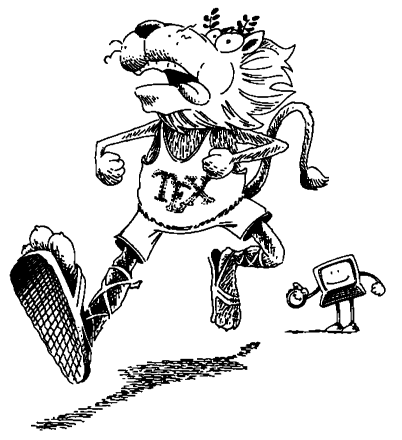
\includegraphics[width = \textwidth]{Chapter6.png}
		\caption{运行\TeX}\label{subfig:2c}
	\end{subfigure}
	\begin{subfigure}[b]{.4\textwidth}
		\centering
		
\includegraphics[width = \textwidth]{Chapter7.png}
		\caption{\TeX 工作原理}\label{subfig:2d}
	\end{subfigure}
	\caption{子图模式测试2:4张图}\label{fig:subfig_test2}
\end{figure}

\section{算法环境}

模板中使用 \texttt{algorithm2e} 宏包实现算法环境。关于该宏包的具体用法请阅读宏包的官方文档。\\
\centerline{-----------$\downarrow$-----------Space Check-----------$\downarrow$-----------}
\begin{algorithm}[!h]
  %\SetAlgoLined
  %\SetAlgoVlined
  \caption{A How to (plain).}
  \KwData{this text}
  \KwResult{how to write algorithm with \LaTeX2e{} }
  
  initialization\;
  \While{not at end of this document}{
    read current\;
    \eIf{understand}{
      go to next section\;
      current section becomes this one\;
    }{
      go back to the beginning of current section\;
    }
  }
\end{algorithm}

\centerline{-----------$\uparrow$-----------Space Check-----------$\uparrow$-----------}

\centerline{-----------$\downarrow$-----------Space Check-----------$\downarrow$-----------}
\RestyleAlgo{ruled}
\begin{algorithm}[!h]
  \caption{A How to (ruled).}
  \KwData{this text}
  \KwResult{how to write algorithm with \LaTeX2e{} }
  
  initialization\;
  \While{not at end of this document}{
    read current\;
    \eIf{understand}{
      go to next section\;
      current section becomes this one\;
    }{
      go back to the beginning of current section\;
    }
  }
\end{algorithm}

\centerline{-----------$\uparrow$-----------Space Check-----------$\uparrow$-----------}

\RestyleAlgo{boxed}
\begin{algorithm}[!h]
  \caption{A How to (boxed).}
  \KwData{this text}
  \KwResult{how to write algorithm with \LaTeX2e{} }
  
  initialization\;
  \While{not at end of this document}{
    read current\;
    \eIf{understand}{
      go to next section\;
      current section becomes this one\;
    }{
      go back to the beginning of current section\;
    }
  }
\end{algorithm}

\RestyleAlgo{boxruled}
\begin{algorithm}[!h]
  \caption{A How to (boxruled).}
  \KwData{this text}
  \KwResult{how to write algorithm with \LaTeX2e{} }
  
  initialization\;
  \While{not at end of this document}{
    read current\;
    \eIf{understand}{
      go to next section\;
      current section becomes this one\;
    }{
      go back to the beginning of current section\;
    }
  }
\end{algorithm}

\section{数学环境}

\subsection{数学符号}

模板定义了一些正体(upright)的数学符号:
\begin{center}
  \begin{tabular}{rl}
    \toprule
    符号                 & 命令 \\
    \midrule
    常数$\eu$     & \verb|\eu| \\
    复数单位$\iu$ & \verb|\iu| \\
    微分符号$\diff$ & \verb|\diff| \\
    $\argmax$         & \verb|\argmax| \\
    $\argmin$         & \verb|\argmin| \\
    \bottomrule
  \end{tabular}
\end{center}

更多的例子:
\begin{equation}
\eu^{\iu\pi} + 1 = 0
\end{equation}
\begin{equation}
\frac{\diff^2u}{\diff t^2} = \int f(x) \diff x
\end{equation}
\begin{equation}
\argmin_x f(x)
\end{equation}

\subsection{定理、引理和证明}

\begin{definition}
  If the integral of function $f$ is measurable and non-negative, we define
  its (extended) \textbf{Lebesgue integral} by
  \begin{equation}
  \int f = \sup_g \int g,
  \end{equation}
  where the supremum is taken over all measurable functions $g$ such that
  $0 \leq g \leq f$, and where $g$ is bounded and supported on a set of
  finite measure.
\end{definition}

\begin{example}
  Simple examples of functions on $\mathbf{R}^d$ that are integrable
  (or non-integrable) are given by
  \begin{equation}
  f_a(x) =
  \begin{cases}
  |x|^{-a} & \text{if } |x| \leq 1,\\
  0 & \text{if } x > 1.
  \end{cases}
  \end{equation}
  \begin{equation}
  F_a(x) = \frac{1}{1 + |x|^a}, \qquad \text{all } x \in \mathbf{R}^d.
  \end{equation}
  Then $f_a$ is integrable exactly when $a < d$, while $F_a$ is integrable
  exactly when $a > d$.
\end{example}

\begin{lemma}[Fatou]
  Suppose $\{f_n\}$ is a sequence of measurable functions with $f_n \geq 0$.
  If $\lim_{n \to \infty} f_n(x) = f(x)$ for a.e. $x$, then
  \begin{equation}
  \int f \leq \liminf_{n \to \infty} \int f_n.
  \end{equation}
\end{lemma}

\begin{remark}
  We do not exclude the cases $\int f = \infty$,
  or $\liminf_{n \to \infty} f_n = \infty$.
\end{remark}

\begin{corollary}
  Suppose $f$ is a non-negative measurable function, and $\{f_n\}$ a sequence
  of non-negative measurable functions with
  $f_n(x) \leq f(x)$ and $f_n(x) \to f(x)$ for almost every $x$. Then
  \begin{equation}
  \lim_{n \to \infty} \int f_n = \int f.
  \end{equation}
\end{corollary}

\begin{proposition}
  Suppose $f$ is integrable on $\mathbf{R}^d$. Then for every $\epsilon > 0$:
  \begin{enumerate}
    \renewcommand{\theenumi}{\roman{enumi}}
    \item There exists a set of finite measure $B$ (a ball, for example) such that
    \begin{equation}
    \int_{B^c} |f| < \epsilon.
    \end{equation}
    \item There is a $\delta > 0$ such that
    \begin{equation}
    \int_E |f| < \epsilon \qquad \text{whenever } m(E) < \delta.
    \end{equation}
  \end{enumerate}
\end{proposition}

\begin{theorem}
  Suppose $\{f_n\}$ is a sequence of measurable functions such that
  $f_n(x) \to f(x)$ a.e. $x$, as $n$ tends to infinity.
  If $|f_n(x)| \leq g(x)$, where $g$ is integrable, then
  \begin{equation}
  \int |f_n - f| \to 0 \qquad \text{as } n \to \infty,
  \end{equation}
  and consequently
  \begin{equation}
  \int f_n \to \int f \qquad \text{as } n \to \infty.
  \end{equation}
\end{theorem}

\begin{proof}
  Trivial.
\end{proof}


\subsection{自定义}

\newtheorem*{axiomofchoice}{Axiom of choice}
\begin{axiomofchoice}
  Suppose $E$ is a set and ${E_\alpha}$ is a collection of
  non-empty subsets of $E$. Then there is a function $\alpha
  \mapsto x_\alpha$ (a ``choice function'') such that
  \begin{equation}
  x_\alpha \in E_\alpha,\qquad \text{for all }\alpha.
  \end{equation}
\end{axiomofchoice}

\newtheorem{observation}{Observation}[chapter]
\begin{observation}
  Suppose a partially ordered set $P$ has the property
  that every chain has an upper bound in $P$. Then the
  set $P$ contains at least one maximal element.
\end{observation}
\begin{proof}[A concise proof]
  Obvious.
\end{proof}

\newtheorem{observationvar2}[observation]{Observationvar2}
\begin{observationvar2}
  Suppose a partially ordered set $P$ has the property
  that every chain has an upper bound in $P$. Then the
  set $P$ contains at least one maximal element.
\end{observationvar2}
\begin{proof}[A concise proof]
  Obvious.
\end{proof}